\clearpage
\section{Arquitectura}
En la figura \ref{arq:arquitectura} se muestra el diagrama de la arquitectura del sistema así como sus componentes.
Posteriormente se encuentra la descripción de cada componente del diagrama.

\begin{figure}[hbtp!]
    \begin{center}
        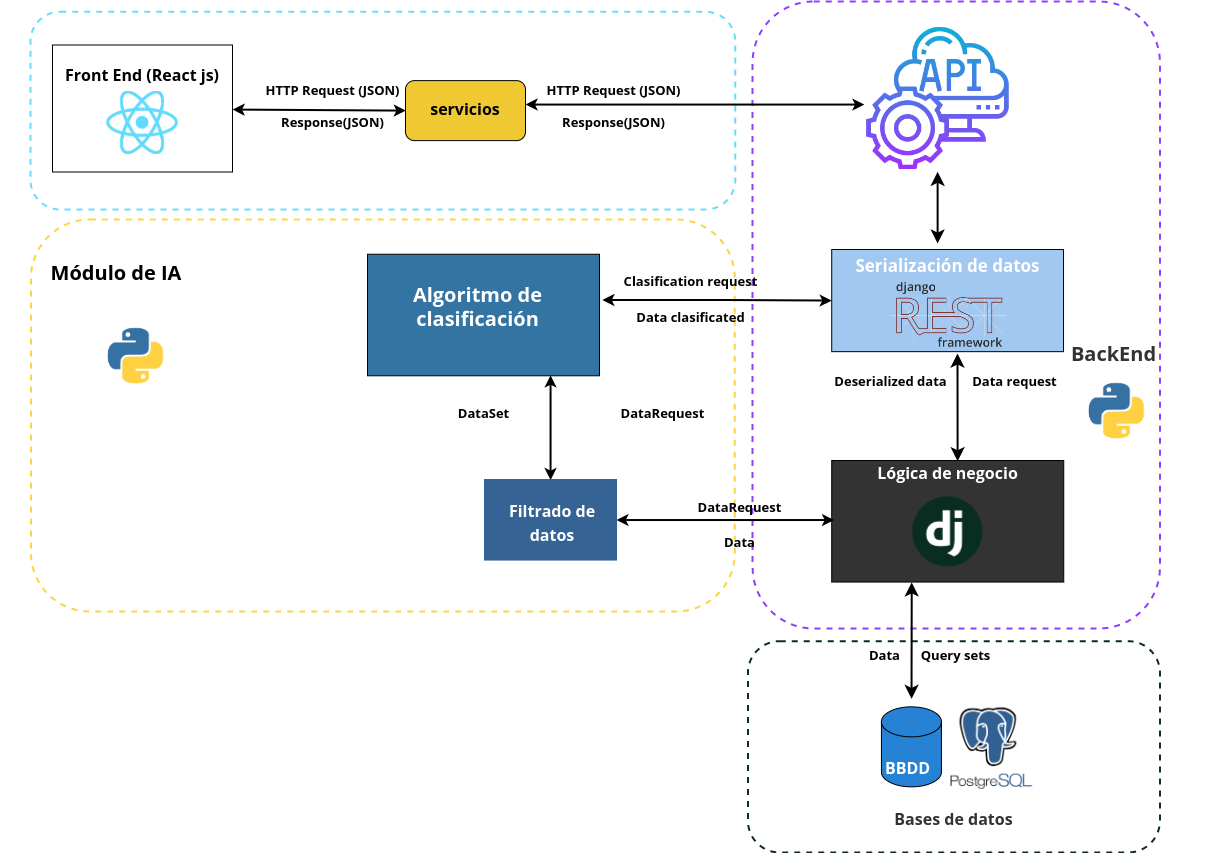
\includegraphics[width=.9\textwidth]{propuesta/imagenes/arqui.png}
    \end{center}
    \caption{Arquitectura del sistema}
    \label{arq:arquitectura}
\end{figure}




\begin{description}
   \item[Front End]  Es el módulo encargado de gestionar las vistas del sistemas para presentarlas a los usuarios, además de encargarse de gestionar el envío de la información de entrada
   para el backend y las solicitudes realizadas a este mismo. Desarrollado con el lenguaje de programación JavaScript y con la librería de React js, lo cual permite
   que desarrollo del módulo en componentes reutilizables y fáciles de montar dentro del sistema para lograr una mejor presentación de pantallas al usuario asi como
   la fácil gestión de la comunicación entre el frontend y el backend.
   
   \item[Backend] Es el módulo principal de gestión de la información del sistema y el cual se encarga de realizar las peticiones de información a la base de datos, crear los registros
   de información, recibir peticiones desde el frontend para acceder a la base de datos, enviar información al frontend y comprobar que la información enviada desde y
   hacia la bese de datos sea correcta de acuerdo a los parámetros establecidos en la creación del modelo de datos. Programado en Python 3 y usando los frameworks Django
   y Django API REST para lograr el manejo de información de acuerdo a las necesidades planeadas para el sistema.
   
   \item[Módulo de IA] Es el módulo encargado de ordenar la información alojada en la base de datos acerca de los perfiles de usuario para la posterior presentación en el sistema. En este
   módulo se aplican algoritmos de clasificación a conjuntos de datos específicos solicitados al módulo de backend para mostrar información útil a los usuarios acerca de
   las vacantes o candidatos registrados en la plataforma para cumplir las necesidades que tenga la empresa del reclutador o las necesidades laborales del candidato.
   
   
   \item[Base de datos] Es la implementación del modelado de datos en el sistema. La implementación de este módulo se realiza en PostgreSQL dada su fiabilidad y flexibilidad de uso en servicios
   de almacenamiento de datos. Este se encarga de almacenar y gestionar la información recolectada por los demás módulos del sistema y así se puedan cumplir con los
   requerimientos establecidos en el modelado de datos, manteniendo la integridad de la información y las necesidades de uso que requiere el sistema para el  funcionamiento
   planeado.
   
\end{description}